%----------------------------------------------------------------------------
\chapter{Cloud-RAN implementáció}\label{sect:CloudImp}
Megismerkedhettünk az előző fejezetben a Cloud-RAN architektúrális felépítésével, ebben a fejezetben bemutatásra kerülnek a főbb implementációs lépések.\cite{BenefitsEricsson}
%----------------------------------------------------------------------------
\section{Cloud-RAN kombináció}
\hspace{2mm} 
\indent A Cloud-RAN architektúrája kombinálhatja a koordináció, központosítás és virtualizáció területén négy fontos előrelépést.\cite{FutureCarrier} \cite{WirelessFull}
\begin{itemize}
\item erőforrások hatékonyabb kezelése: költséghatékonyabb processzor megosztás,
\item méretezhetőség: hardver kapacitás rugalmasabb növelése,
\item rétegek együttműködése: pl. alkalmazás réteg és RAN közötti szorosabb együttműködés,
\item spektrális hatékonyság
\end{itemize}
Fontos megértenünk, hogy a kombináció melyik tagja miben jelent előrelépést. Ezeket az implementációs aspektusokat \figref{imp_aspects}-es táblázattal szemléltethetjük.
\begin{figure}[!ht]
\centering
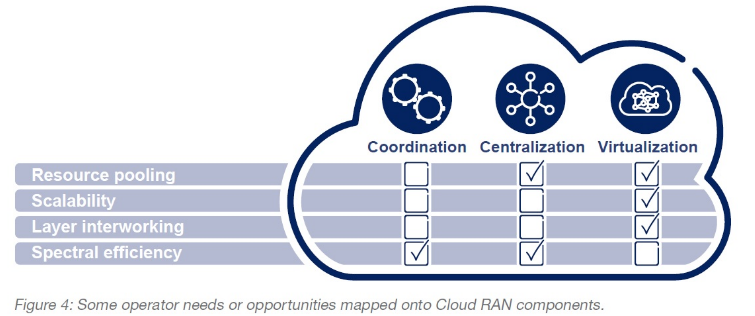
\includegraphics[width=\textwidth, keepaspectratio]{figures/imp_aspects.png}
\caption{Az implementációs aspektusok.} 
\label{fig:imp_aspects}
\end{figure} 
%----------------------------------------------------------------------------
\section{Virtualizáció a Cloud-RAN-ban}
\hspace{2mm}
\indent Itt a rádiós hozzáférési protokoll által támasztott valós-idejűség követelményei jelentik az alapvető különbséget (számos szinkronizációs folyamat, amely a protokoll teljesítményét biztosítja, mikro-vagy nano szekundumos sebesség szintjén kell legyen). 
Érdemes megjegyezni, hogy nem szükséges az összes RAN funkciót virtualizálni ahhoz, hogy a Cloud-RAN adta lehetőségeket kiaknázzuk. Így többek között képes biztosítani az elszigeteltséget, a méretezhetőséget, valamint rugalmasságot az RRC protokoll réteg szintjén.
%----------------------------------------------------------------------------
\section{Centralizáció a Cloud-RAN-ban}
\hspace{2mm}
\indent A Cloud-RAN-nal dolgozó központosított bázisállomás egyszerűsíti a hálózati menedzsmentet és lehetővé teszi az erőforrás összevonást (resource pooling), illetve a rádiós erőforrások koordinációját. A pooling, vagy a statisztikai multiplexálás egy végrehajtási platformot nyújt, amellyel ugyanazon feladatok láthatók el kevesebb hardver és kapacitás felhasználása mellett. A központosítás számos előnye közül érdemes kiemelni, hogy forgalomirányításnak és a mobilitás központosításnak köszönhetően kevesebb a handover hiba, illetve a heterogén hálózatokban kevesebb jelhiba lép fel. Ezen kívül a centralizáció azt is eredményezi, hogy az X2 interfész végpontjai közötti távolság megrövidül, így végső soron gyorsabb (kisebb késleltetés miatt) lesz az X2 interfészen való kommunikáció.\cite{BenefitsFujitsu}
%----------------------------------------------------------------------------
\section{Koordináció a Cloud-RAN-ban}
\hspace{2mm}
\indent A központosított koordináció különösen alkalmas a hálózat teljesítményének javítására, kiemelendő a handoverek, a carrier aggregáció és az interferencia menedzsment területén. Ezenfelül a többszintű koordináció olyan esetekben is lehetséges, amikor a centralizáció a rádiós protokoll magasabb rétegeire korlátozódik.\cite{BenefitsEricsson}\cite{NokiaSingle}
%----------------------------------------------------------------------------
\section{Implementációs nehézségek}
\hspace{2mm}
\indent A tiszta szoftverdefiniált rádiós rendszerben, az összes rádió funkció egy GPP-n (General Purpose Processor, általános célú processzor) fut. A virtuális környezet folyamatos interakcióban van a fizikai erőforrásokkal direkten vagy valamilyen emulációs rétegen keresztül. Ez virtuális szoftver eladható akár egy szolgáltatásként, mely valamilyen felhőben van kontrollálva. Ezáltal beszélhetünk RANaaS-ról azaz RAN as a Service-ről vagy általánosabban NaaS-ról, Network as a Service. Az ilyen hálózatoknak már több prototípusa is elkészült, melyekből rengeteg tanulságot vonhattunk le. (A legnagyobb kihívást jelenleg a csomagok késői megérkezései okozzák, melyek nagy hatással vannak a felhasználi élményre.)\cite{Architecture}\cite{ImplementationIssues}\cite{ImplementingGPP}
\begin{figure}[!ht]
\centering
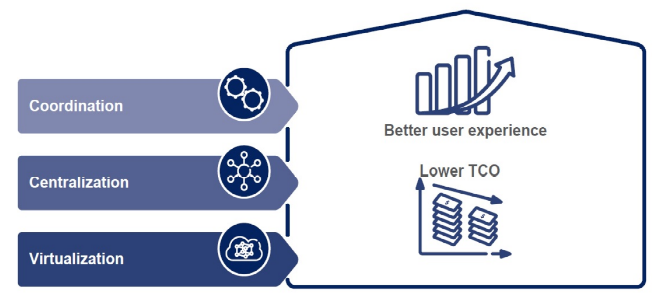
\includegraphics[width=\textwidth, keepaspectratio]{figures/cool.png}
\caption{A Cloud-RAN eszköszök és előnyök} 
\label{fig:cool}
\end{figure}
%----------------------------------------------------------------------------
\section{Záró gondolat}
\indent A Cloud-RAN új környezetében tehát lehetőség van arra, hogy az üzemeltetők nagyobb hálózati kapacitást és lefedettséget biztosíthassanak az előfizetőik számára kisebb összköltség (total cost of ownership, TCO) mellett, lsd \figref{cool}-es ábra. Mindez alapja lehet a jövő szélessávú mobilhálózatainak. Nyilván felmerül a kérdés, hogy vajon mikor kerül sor a Cloud-RAN ipari léptékű megvalósítására? A mobil hálózati architektúra forradalma a közelgő virtualizációval (Network functions virtualization, NFV) várható és a szolgáltatók a folyamatos fejlődés útján bizonyára nyitni fognak a Cloud-RAN koncepció irányába. 